% Intended LaTeX compiler: pdflatex
\documentclass{scrartcl}
    \usepackage[dvipdfmx]{geometry}
		\usepackage[utf8]{inputenc}
		\usepackage[dvipdfmx]{graphicx}
		\usepackage[dvipdfmx]{color}
		\usepackage[backend=biber,bibencoding=utf8]{biblatex}
		\usepackage{url}
		\usepackage{indentfirst}
		\usepackage[normalem]{ulem}
		\usepackage[dvipdfmx]{hyperref}
		\usepackage{longtable}
		\usepackage{minted}
		\usepackage{fancyvrb}
		\bibliography{reference}
\author{情報科学類二年 江畑 拓哉(201611350)}
\date{}
\title{seis-ml-api中間レポート}
\begin{document}

\maketitle
\tableofcontents


\section{前書き}
\label{sec:org274100e}
 このレポートは情報特別演習における中間レポートとして編集したものだ。但しここにおける中間レポートの意味は、今後の方針を明確にするための現在までに仮決定された事項をまとめるということにある。即ちここに書かれるものは、これまでに実験した、学習した内容ではなく、それを総括して最終的に今後使用する可能性のあるものに限られる。\\
 更に既存のツールを用いたツールで実験した結果や機械学習の詳細な導出については別紙に実験レポートとして作成する。\\

\section{seis-ml-api概要}
\label{sec:org6b3bb48}
 このapi(と仮定する)は、この情報特別演習を受けた我々の追加目標であり、私の課題である。我々は3人でグループを組んでいるが、それぞれにテーマを設けて研究を行っており、私は二人の研究成果をまとめる他に、それを活用して独自にこの api を作成することになっている。\\
 この api の目指すものは未確定部分が多いものの(詳しい目標については発案者に質問いただきたい)現在私が作成を行っているものは、”時系列データ分析とランダムフォレストを利用した、相関に基づく時系列予測”とでも言うべきものである。そしてこの抽象的なチャートについては以下の通りである。\\
\begin{figure}[htbp]
\centering
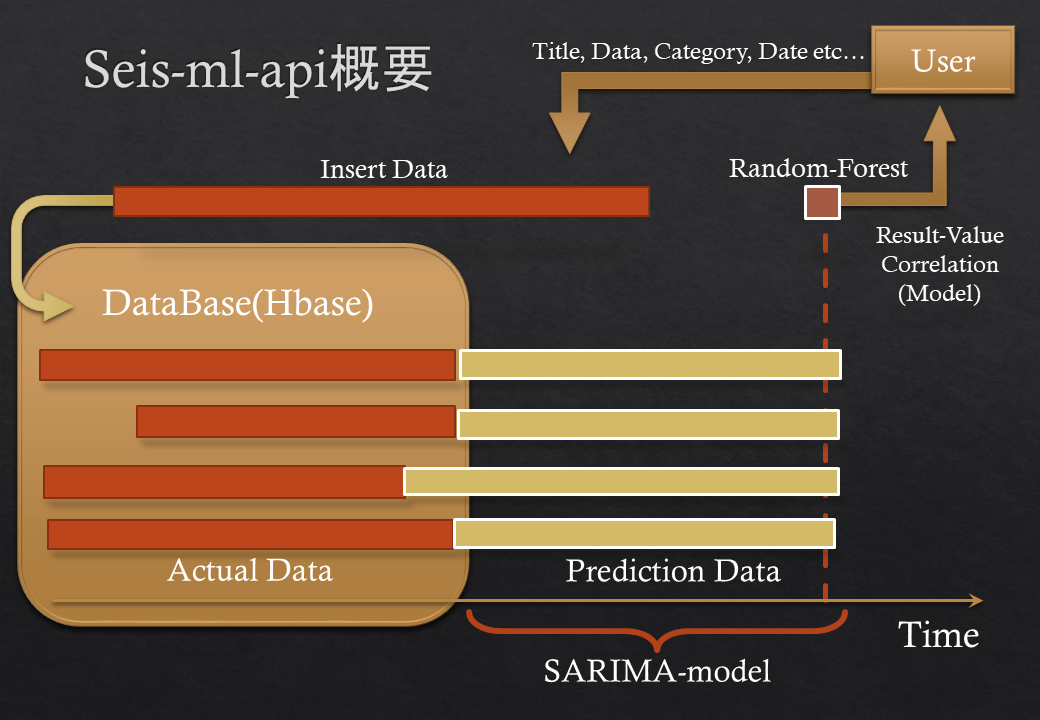
\includegraphics[width=15cm]{./idea-1.png}
\caption{seis-ml-apiの抽象的チャート}
\end{figure}

例えば、ユーザーから2015年までの株価データの入った ”( csv )ファイル(タイトル)” と、 "それの属するカテゴリ" 、 そして必要なデータの2017年12月といった "時間データ" 転送されたとする。まずデータベースに登録されている指定されたカテゴリに属するデータについて、 SARIMA モデルを用いて時系列解析を行う。そして指定された時間データまでの値を予測する。次にこれらの予測データに加え与えられたファイルを用いてランダムフォレストによる回帰解析を行い、指定された時間データの値を欠損値補完する。そして得られた "補完データ" と "相関についてのデータ(相関の高い順3つのタイトルなど) " をユーザに返し、ユーザから与えられたファイルは指定されたカテゴリに基づいてデータベースに保存する。\\

つまり必要となるデータは、\\
\begin{itemize}
\item タイトル\\
\item 時系列データ\\
\item そのデータの属するカテゴリ\\
\item 欲しい時間データ\\
\end{itemize}

 そして返すデータは、\\
\begin{itemize}
\item 補完データ\\
\item 相関についてのデータ\\
\end{itemize}

 ということになる。\\

\subsection{実験に用いるデータ}
\label{sec:orga6354a5}
 今回実験に用いるデータについて明確にするため、ここで今後活用して行くデータの入手先を明確にしておく。これからまず手に入れるであろうデータのカテゴリは、日本の経済系にあるデータで、例えば日経平均株価がそれに当たる。そして挑戦できるならばそれに加えて日本の人口のデータも検討してみたいと考えている。\\
\begin{itemize}
\item google finance\\
日本のデータをcsvで入手することは困難だが、海外のデータは容易に手に入る。\\
\item Quandl\\
 ほとんどすべてのデータはここで手に入る。但し、どうやら長期間のデータは乏しいようである。主にはこちらから得た株価データを用いて分析を行う。\\
\item 総務省統計データ\\
 あまりめぼしいデータはないが、ゼロというわけではないため活用していきたい。\\
\end{itemize}

\section{機械学習部分(時系列解析)}
\label{sec:orgfe2b4d1}
   実験に関しては別紙にまとめて示す。\\
   時系列解析に用いるモデルは季節的自己回帰和分移動平均モデルことSARIMAモデルを用いる。\\
SARIMAとは、 Seasonal ARIMAモデルであり、これは季節性のあるモデルとARIMAモデルを組み合わせたものである。\\
   Seasonal部分は、ARIMAモデルをある周期区間に適用したもので、これを下記のARIMAモデルと組み合わせることで、ある程度の周期性を持たせることができる。例えば、毎年同じような経営方針の会社があれば、このSeasonal部分が組み込まれることで、より現実的な値を返すことができるだろう(そしてこのような周期性はおおよそどのような国でも見受けられるようであることを別紙に記載する実験により予測された)。\\
   ARIMAモデルとは、 Autoregressive Integrated Moving Average Model である。\\
   Autoregressive とは、重回帰のようなアルゴリズムを用いた自己回帰法である。例えば \(a->b->c\) という遷移があれば、 \(b->c->d\) であると考えられるようなものである。\\
   Moving Average とは、移動平均という意味であるが、これは簡単には説明しづらいものがあるため、抽象的な考え方で説明を行いたいが、その前にこれが移動平均と呼ばれる所以を説明する。ある区間の平均値を求めた際に、その平均値に対して計算に用いる要素は区間の中心ではなく、区間の最新部分である。つまりは平均値を格納する位置を移動しているといったことが移動平均と呼ばれる所以の一つなのだ。そして、MAモデルの重大な特徴として、このモデルはある時系列データそのものではなく、先程求めた移動平均とそれが格納されている時系列データの要素との差、つまり移動平均誤差について所謂回帰の議論を行うというものである。\\

\section{機械学習部分(ランダムフォレスト)}
\label{sec:org058ee37}
実験に関しては別紙にまとめて示す。\\
上の機械学習部分に関して、求めたい時系列タイトルを除いた関連データの時系列解析が終わったところで、呼び出されることになるこのアルゴリズムは、複数の低級な決定木を多く生やすことでデータの分析をするもので、今回はこれを回帰の欠損補完に用いることとする。\\
ランダムフォレストの説明に移る前に決定木、特にその回帰について説明する。\\

\subsection{決定木}
\label{sec:org2457ac4}
 決定木とは、複数の説明変数を持つデータセットに対して、もっとも議論のデータセットを分割できるように分け、分けた要素について再帰的に同様の処理を行うという分類・回帰法であり、これによってどのような条件でどのような目的値がふさわしいのかを求めることができる。この分割における最適化を用いる方法には、例えばエントロピーやジニ係数、尤離度(逸脱度)などの所謂”分離度”を測る式を用いる。\\
 後に言う、高い・低い決定木とはこの分割の回数を意味し、高い決定木であればあるほどより細かい分類・回帰が可能となり、低い決定木では大まかな概要を掴むことができる。\\

\subsection{ランダムフォレスト }
\label{sec:org555b5ad}
 ランダムフォレストとは、与えられたデータセットの中から任意のデータを抽出して集めた複数のデータセットについて低い決定木を並行して行い、それによって求められた結果の集合に基づいて元のデータセットの分析をするというものである。今回の回帰を用いた欠損補完においては、決定木のうちの回帰木を用いて求まった値の平均を取りそれを参考にすることで欠損補完を行う。そして、その結果と計算に用いられなかった残りのデータを用いることで説明変数の重要度を探ることができる。\\

\section{データベース部分}
\label{sec:orgbf37af6}
 データベース部分に関してはApach HBaseを用いた大規模スケールの箱を作る予定である。大規模データベースの中身の設計については割愛する(データの安全保障や機械学習の制度などの問題から、データを増やし過ぎることが厳しい)が、 hbase のクエリと csv のファイルとつなげる部分や、同一データの判定などの機能を作成する必要があるためデータベースとの接合に関しては未だ展望が見えていないのが現実である。\\

\section{参考文献}
\label{sec:org9906ee8}
以下にそれぞれで用いた参考文献を示す。なお、これらの文献は今後より深く読み進めていく予定である。\\
\begin{itemize}
\item SARIMAモデルについて \cite{sarima01} \cite{sarima02} \cite{sarima03} \cite{sarima04} \cite{sarima05}\\
\item RandomForestについて \cite{rf01} \cite{rf02} \cite{rf03} \cite{rf04} \cite{rf05} \cite{rf06} \cite{rf07} \cite{Breiman:2001:RF:570181.570182} \cite{rf08} \cite{rf09}\\
\item 決定木について \cite{tree01}\\
\item データベースについて \cite{hbase01} \cite{hbase02} \cite{hbase03}\\
\end{itemize}

\printbibliography\\
\end{document}